\documentclass[tikz, border=10pt]{standalone}
\usetikzlibrary{shapes}
% standalone document class allows us to create documents that consist of a
% single drawing and cuts the PDF document to the actual content
% 
% border=10pt, for a small margin
\begin{document}
%%%%\begin{tikzpicture}
%%%%	\draw[thin, dotted, step=0.5] (-3, -3) grid (3, 3);
%%%%	\draw[->] (-3, 0) -- (3, 0);
%%%%	\draw[->] (0, -3) -- (0, 3);
%%%%	\draw[very thin, blue] (-2, -2) -- (-2, 2) -- (2, 2) -- (2, -2) -- cycle;
%%%%	\draw[very thick, red] (-2, -2) circle (1) (-2, 2) circle (1) (2, 2) circle (1) (2, -2) circle (1);
%%%%	\draw[very thick, cyan] (0:2) -- (60:2) -- (120:2) -- (180:2) -- (240:2) -- (300:2) -- cycle;
%%%%	% tizke use (angle:distance) syntax for polar coordinate
%%%%	\draw[very thick, green] (-3, -1) -- +(1, 0) -- +(2, 2) -- +(4, 2) -- +(5, 0) -- +(6, 0);
%%%%	% relative position with `+`
%%%%	\draw[very thick, magenta] (-3, -1) -- ++(1, 0) -- ++(1, 2) -- ++(2, 0) -- ++(1, -2) -- ++(1, 0);
%%%%	% `++` double plus signs 
%%%%\end{tikzpicture}
% draw syntax
% \draw[<style>] <coordinate> <picture element> <coordinate> ... ;
% `step` argument default to 1
% `--` shortcut stands for a line
% `->` shortcut stands for a arrow

%%%%\begin{tikzpicture}
%%%%	[x={(0.86cm, 0.5cm)}, y={(-0.86cm, 0.5cm)}, z={(0cm, 1cm)}]
%%%%	\draw[very thick, blue] (-2, -2, 0) -- (-2, 2, 0) -- (2, 2, 0) -- (2, -2, 0) --cycle;
%%%%	\draw[->] (0, 0, 0) -- (2.5, 0, 0)  node [right] {x};
%%%%	\draw[->] (0, 0, 0) -- (0, 2.5, 0)  node [left] {y};
%%%%	\draw[->, dashed] (0, 0, 0) -- (0, 0, 2.5) node [above] {z};
%%%%	\draw circle (2);
%%%%\end{tikzpicture}

%%%%\begin{tikzpicture}[x=1cm, y=1cm]
%%%%	\draw[shading=ball, ball color=yellow] (0, 0) circle[radius=2];	
%%%%	%\draw[fill=black] (-0.5, 0.5, 0) ellipse [x radius=0.2, y radius=0.4];
%%%%	\draw[shading=ball, ball color=black] (-0.5, 0.5, 0) ellipse [x radius=0.2, y radius=0.4];
%%%%	\draw[shading=ball, ball color=black] (0.5, 0.5, 0) ellipse [x radius=0.2, y radius=0.4];
%%%%	\draw[very thick] (-1, -1) arc [start angle=185, end angle=355, x radius=1, y radius=0.5];
%%%%\end{tikzpicture}

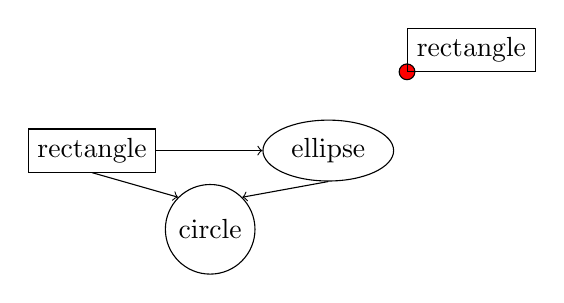
\begin{tikzpicture}
	%\draw (4, 2) node[draw, color=red, fill=yellow, text=blue] {TikZ};
	% `draw` draw the border
	\node (r) at (0, 1)		[draw, rectangle]	{rectangle};
	\node (c) at (1.5, 0)	[draw, circle] 		{circle};	
	\node (e) at (3, 1)		[draw, ellipse]		{ellipse};
	\draw[->] (r.east)	--	(e.west);
	\draw[->] (r.south) --	(c.north west);
	\draw[->] (e.south) --	(c.north east);
	\draw[fill=red] (4, 2) circle[radius=0.1];
	%\node at (4, 2)			[draw, rectangle]	{rectangle};
	\node at (4, 2)			[draw, rectangle, anchor=south west] {rectangle};
\end{tikzpicture} 

\end{document}
